\documentclass[11pt,a4paper]{article}
\usepackage[margin=2.3cm]{geometry}
\usepackage{amsmath,amssymb,bm}
\usepackage{siunitx}
\usepackage{booktabs}
\usepackage{nicefrac}
\usepackage{graphicx}
\usepackage{tikz}
\usetikzlibrary{arrows.meta,calc,positioning,patterns}
\usepackage{pgfplots}
\pgfplotsset{compat=1.17}
\usepackage{enumitem}
\usepackage{float}
\tikzset{capt/.style={text width=5.2cm,align=center}}
\usepackage[colorlinks=true,linkcolor=blue!60!black,urlcolor=blue!60!black]{hyperref}
\usepackage{fancyhdr}
\usepackage{tcolorbox}
\tcbuselibrary{skins,breakable}
\sisetup{per-mode=symbol,detect-all}

\newtcolorbox{keybox}[1]{title={#1},colback=blue!4,colframe=blue!50!black,fonttitle=\bfseries,breakable}
\newtcolorbox{examplebox}[1]{title={#1},colback=green!4,colframe=green!40!black,fonttitle=\bfseries,breakable}
\newtcolorbox{aerobox}[1]{title={#1},colback=orange!5,colframe=orange!60!black,fonttitle=\bfseries,breakable}

\pagestyle{fancy}
\fancyhf{}
\lhead{
\includegraphics[height=0.6cm]{logos/itu_logo_laci.pdf}\ \ UCK 364E Design of Machine Elements}
\setlength{\headheight}{20pt}
\rhead{Lecture 6 -- Notes}
\cfoot{\thepage}

\title{\textbf{UCK 364E Design of Machine Elements}\\[4pt]
\Large Lecture 6: Tension and Shear Joints\\[2pt]
\large What the fastener does once it is in a joint}
\author{Prof.\ Dr.\ Onur Tunçer\\ Department of Aeronautical Engineering, Istanbul Technical University}
\date{Fall 2026}


\begin{document}
\maketitle

\section*{Learning objectives}
By the end of this lecture you should be able to:
\begin{enumerate}[nosep]
  \item Draw the joint diagram for a preloaded joint and read the load split off it.
  \item Compute the bolt and member loads under an external tensile load, and the margins against
        \emph{yielding} and against \emph{separation}.
  \item Compute the fatigue factor of a preloaded bolt, and explain why the alternating stress
        depends on $C$ and not on the preload --- and what the preload is therefore for.
  \item Choose a preload, knowing what bounds it from above and from below.
  \item Check a shear joint against all four of its failure modes and state which one governs.
  \item Explain what edge distance and pitch are protecting against, and size them.
  \item Show that fasteners in a line do not share load equally, and say which one cracks first.
  \item Choose between solid, blind and pin-and-collar fasteners, read a rivet's alloy from
        its head, and state the driving dimensions that make the shop head an inspection.
  \item Analyse an eccentrically loaded bolt group and find the critical bolt.
  \item Apply the combined tension--shear interaction equation, and say why the exponents depend on
        where the shear plane falls.
  \item Specify the grip length of a bolt in shear, and say what goes wrong if you do not.
\end{enumerate}

\section{Why this lecture exists}

Lecture 5 gave you the fastener. This lecture gives you the \emph{joint}, and the two are not the
same subject. A bolt that is perfectly specified --- right thread, right class, right preload ---
will still fail if the joint around it was analysed in the wrong direction.

\medskip
There are exactly two directions, and they have almost nothing in common:

\begin{center}\footnotesize
\begin{tabular}{@{}p{3.1cm}p{5.6cm}p{6.6cm}@{}}
\toprule
 & \textbf{Tension joint} & \textbf{Shear joint}\\
\midrule
The load is & along the bolt axis & across it\\[2pt]
What carries it & the \emph{clamp}, until the joint separates & the bolt shank in shear, and the
  plate in bearing\\[2pt]
Preload is & the whole design variable & largely irrelevant to strength\\[2pt]
What you check & yielding, separation, fatigue & bolt shear, bearing, net tension, shear-out\\[2pt]
What usually governs & fatigue & bearing, or the plate\\[2pt]
Fails by & the bolt stretching or the joint opening & the hole elongating, or the plate tearing\\
\bottomrule
\end{tabular}
\end{center}

\medskip
And one thing they \emph{do} have in common: a \textbf{fitting factor of 1.15}, applied on top of
the ultimate factor of 1.5, on every joint, fitting and bearing surface (CS/FAR 25.625). Lecture 1
introduced it; from here on it is in every margin you write.

\begin{keybox}{A word about which bolts are which}
A bolt in a well-designed \emph{tension} joint is preloaded hard and never sees the external load
directly. A bolt in a \emph{shear} joint is preloaded too --- but the preload is there to stop
fretting and to keep the joint rigid, not to carry the load. Aerospace shear joints are routinely
analysed as if the preload were zero, because friction is not a certifiable load path. The bolt
bears, and you size it for bearing.
\end{keybox}

\section{The preloaded joint under tension}
\label{sec:tension}

\subsection{The joint diagram}

Lecture 5 established the two stiffnesses --- $k_b$ for the bolt, $k_m$ for the clamped members ---
and the joint constant
\[
C=\frac{k_b}{k_b+k_m}.
\]
Everything in this section is a consequence of one picture.

\begin{figure}[H]\centering
\resizebox{0.86\textwidth}{!}{% The joint diagram. Numbers are the M10 joint of Lecture 5: ki=485, km=1936 kN/mm, Fi=36.1 kN, P=20 kN.
\begin{tikzpicture}[>=Latex,line join=round]
\tikzset{
  bolt/.style={blue!60!black,line width=1.4pt},
  memb/.style={orange!75!black,line width=1.4pt},
  thin2/.style={gray!60,thin},
  dimn/.style={<->,gray!70!black,thin},
  lb/.style={font=\scriptsize},
  key/.style={font=\scriptsize,align=left}
}
\def\xs{70}      % mm  -> cm
\def\ys{0.11}    % kN  -> cm
\pgfmathsetmacro\db{0.0744*\xs}     % bolt stretch at preload
\pgfmathsetmacro\dm{0.0186*\xs}     % member squash at preload
\pgfmathsetmacro\Fi{36.1*\ys}
\pgfmathsetmacro\dd{0.00826*\xs}    % extra deflection under P
\pgfmathsetmacro\Fb{40.1*\ys}
\pgfmathsetmacro\Fm{20.1*\ys}
\pgfmathsetmacro\base{\db+\dm}
\pgfmathsetmacro\Fmid{(\Fb+\Fm)/2}

% axes
\draw[->,black!70] (-0.3,0) -- (\base+2.6,0);
\node[font=\scriptsize,anchor=north] at (\base+1.9,-0.08) {deflection $\delta$};
\draw[->,black!70] (0,-0.3) -- (0,\Fi+1.9) node[anchor=north west,font=\scriptsize,rotate=90,xshift=-4pt] {force};

% ---- the two springs at preload ----
\draw[bolt] (0,0) -- (\db,\Fi);
\draw[memb] (\base,0) -- (\db,\Fi);
\node[lb,text=blue!60!black,anchor=south east,rotate=37] at (\db*0.55,\Fi*0.55) {bolt, slope $k_b$};
\node[lb,text=orange!75!black,anchor=south west,rotate=-72] at (\db+\dm*0.42,\Fi*0.52) {member, slope $k_m$};

% preload level
\draw[thin2,dashed] (0,\Fi) -- (\db,\Fi);
\node[lb,anchor=east] at (-0.1,\Fi) {$F_i$};
\fill[black] (\db,\Fi) circle (1.8pt);

% ---- after the external load P is applied ----
\draw[bolt,dashed,opacity=0.9] (\db,\Fi) -- (\db+\dd,\Fb);
\draw[memb,dashed,opacity=0.9] (\db,\Fi) -- (\db+\dd,\Fm);
\fill[blue!60!black] (\db+\dd,\Fb) circle (1.8pt);
\fill[orange!75!black] (\db+\dd,\Fm) circle (1.8pt);

% the split of P
\draw[thin2,dashed] (\db+\dd,\Fb) -- (\base+1.95,\Fb);
\draw[thin2,dashed] (\db+\dd,\Fm) -- (\base+1.95,\Fm);
\draw[thin2,dashed] (\db+\dd,\Fi) -- (\base+1.95,\Fi);

\draw[dimn,blue!60!black] (\base+0.30,\Fi) -- (\base+0.30,\Fb);
\node[lb,text=blue!60!black,anchor=west] at (\base+0.40,\Fb+0.02) {$\Delta F_b = CP$};
\draw[dimn,orange!75!black] (\base+0.30,\Fm) -- (\base+0.30,\Fi);
\node[lb,text=orange!75!black,anchor=west] at (\base+0.40,\Fm-0.02) {$\Delta F_m = -(1-C)P$};
\draw[dimn,black!75] (\base+1.95,\Fm) -- (\base+1.95,\Fb);
\node[lb,anchor=west] at (\base+2.05,\Fmid) {$P$};

% deflections at preload
\draw[dimn] (0,-0.45) -- (\db,-0.45);
\node[lb,anchor=north] at (\db/2,-0.48) {$\delta_b = F_i/k_b$};
\draw[dimn] (\db,-0.45) -- (\base,-0.45);
\node[lb,anchor=north] at (\db+\dm/2,-0.48) {$\delta_m$};

% the reading
\node[key,anchor=north west,text width=7.4cm] at (-0.2,-1.25)
 {\textbf{Read it as a lever.} The two springs share the external load in proportion to their
  stiffnesses. The \emph{members} are the stiff one here, so they shed most of $P$ and the bolt
  feels only $C=k_b/(k_b+k_m)$ of it. For this joint $C=0.20$: a \SI{20}{kN} external load adds
  only \SI{4}{kN} to the bolt.};

\end{tikzpicture}
}
\caption{The joint diagram. Preload stretches the bolt and squashes the members; an external load
$P$ stretches the bolt \emph{further} and lets the members relax. The two effects must be equal in
deflection, which is what splits $P$.}
\label{fig:jointdiag}
\end{figure}

When an external tensile load $P$ is applied to the joint, bolt and members must deflect together.
The bolt takes the fraction $C$ and the members shed the rest:
\[
\boxed{\;F_b = F_i + C\,P\;}
\qquad\qquad
\boxed{\;F_m = F_i - (1-C)\,P\;}
\]
with $F_b$ the total bolt load and $F_m$ the clamping force left between the members. Note the
signs: \textbf{the bolt load barely rises, and the clamp force falls fast}. For the M10 joint of
Lecture 5, with $C=0.20$, a \SI{20}{kN} external load adds \SI{4}{kN} to the bolt and removes
\SI{16}{kN} of clamp.

\subsection{Two things can go wrong, and they pull in opposite directions}

\paragraph{Yielding.} The bolt stress must stay below the proof strength:
\[
\sigma_b=\frac{F_i+CP}{A_t}\le S_p
\qquad\Longrightarrow\qquad
\boxed{\;n_p=\frac{S_pA_t-F_i}{C\,P}\;}
\]
Raise the preload and this margin falls.

\paragraph{Separation.} The joint opens when the members stop pressing on each other, $F_m=0$:
\[
P_0=\frac{F_i}{1-C}
\qquad\Longrightarrow\qquad
\boxed{\;n_0=\frac{F_i}{P\,(1-C)}\;}
\]
Raise the preload and this margin \emph{rises}. The two requirements squeeze the preload from
opposite sides, which is why $F_i$ is a design decision and not a default.

\begin{aerobox}{Separation is not a serviceability issue. It is a cliff.}
A joint that has separated is a different machine. The members no longer share the load, so the
bolt carries \emph{all} of $P$ instead of $CP$ --- an instant multiplication by $1/C$, which for a
typical joint is a factor of four to eight. Everything you calculated about fatigue is void from
that moment. We put a number on this in Example 6.1.
\end{aerobox}

\section{Fatigue of the preloaded joint}
\label{sec:boltfatigue}

This is the calculation Lecture 5 kept deferring, and it is the one that usually governs.

\medskip
Take an external load fluctuating between $0$ and $P$. The bolt sees only $C$ of it, so
\[
\sigma_a=\frac{C\,P}{2A_t},
\qquad
\sigma_i=\frac{F_i}{A_t},
\qquad
\sigma_m=\sigma_a+\sigma_i .
\]
The load line on a Goodman diagram therefore starts at $(\sigma_i,0)$ and rises at
$45^\circ$ --- because every increment of alternating stress brings an equal increment of mean
stress. Intersect it with the Goodman line $\sigma_a/S_e+\sigma_m/S_{ut}=1$:
\[
\frac{\sigma_a}{S_e}+\frac{\sigma_i+\sigma_a}{S_{ut}}=1
\qquad\Longrightarrow\qquad
\sigma_{a,\text{lim}}=\frac{S_e\,(S_{ut}-\sigma_i)}{S_{ut}+S_e}
\]
\[
\boxed{\;n_f=\frac{\sigma_{a,\text{lim}}}{\sigma_a}
=\frac{S_e\,(S_{ut}-\sigma_i)}{\sigma_a\,(S_{ut}+S_e)}\;}
\]

\begin{keybox}{The thing students get backwards}
Look hard at $\sigma_a = CP/2A_t$. \textbf{It does not contain $F_i$.} Once the joint is closed,
increasing the preload does \emph{not} reduce the alternating stress in the bolt --- it only raises
the mean stress, which by Goodman makes $n_f$ slightly \emph{worse}.

\medskip
So why preload hard? Because of the cliff. The preload's job is to \textbf{guarantee the joint never
opens}, and the alternating stress is small only while that is true. Preload does not reduce the
fatigue load; it protects the condition under which the fatigue load is small. Those are different
statements and only the second one is true.

\medskip
What \emph{does} reduce $\sigma_a$ is reducing $C$ --- a more flexible bolt, stiffer members, a
washer. That is the whole argument of \S10.4 of Lecture 5, and it is why a long slender bolt
through a stiff flange is the classic fatigue-tolerant joint.
\end{keybox}

\begin{examplebox}{Example 6.1 --- the M10 joint of Lecture 5, now with an external load}
The same joint: M10$\times$1.5 class 10.9, $A_t=\SI{58.0}{mm^2}$, $S_p=\SI{830}{MPa}$,
$S_{ut}=\SI{1040}{MPa}$; $k_b=\SI{485}{kN/mm}$, $k_m=\SI{1936}{kN/mm}$ so $C=0.200$. Proof load
$F_p=S_pA_t=\SI{48.1}{kN}$ and preload $F_i=0.75F_p=\SI{36.1}{kN}$. The joint carries an external
load per bolt fluctuating from $0$ to $P=\SI{20}{kN}$.

\medskip
\textbf{Static.} $F_b=F_i+CP=36.1+0.2(20)=\SI{40.1}{kN}$, so $\sigma_b=\SI{692}{MPa}$.
\[
n_p=\frac{48.1-36.1}{0.2\times20}=\mathbf{3.00},
\qquad
n_0=\frac{36.1}{20(1-0.2)}=\mathbf{2.26}
\]

\textbf{Fatigue.} With $S_e=\SI{162}{MPa}$ (fully corrected, rolled thread, class 10.9 ---
Shigley Table 8-17):
\[
\sigma_a=\frac{0.2\times20\,000}{2\times58}=\SI{34.5}{MPa},
\qquad
\sigma_i=\frac{36\,100}{58}=\SI{622}{MPa}
\]
\[
n_f=\frac{162\,(1040-622)}{34.5\,(1040+162)}=\mathbf{1.63}
\]

\medskip
\textbf{Fatigue governs}, at 1.63. Now the cliff. Suppose the joint separates --- the preload was
lost, or $P$ exceeded $P_0=\SI{45.1}{kN}$. The bolt then carries all of $P$:
\[
\sigma_a=\frac{20\,000}{2\times58}=\SI{172}{MPa}
\qquad(\text{exactly }1/C=5\times\text{ the closed-joint value})
\]
and with $\sigma_m=\sigma_a$, Goodman gives
$n=\left(\tfrac{172}{162}+\tfrac{172}{1040}\right)^{-1}=\mathbf{0.81}$.

\medskip
\emph{The joint that had a comfortable fatigue margin fails in fatigue the moment it opens.} That
is what the preload is buying, and it is the only thing it is buying.
\end{examplebox}

\subsection{Choosing the preload}

Run Example 6.1 again at three preloads and the structure of the decision appears:

\begin{center}\small
\begin{tabular}{@{}lccc@{}}
\toprule
Preload & $n_p$ (yield) & $n_0$ (separation) & $n_f$ (fatigue)\\
\midrule
$0.90F_p$ & 1.20 & 2.71 & 1.14\\
$\mathbf{0.75F_p}$ & \textbf{3.00} & \textbf{2.26} & \textbf{1.63}\\
$0.50F_p$ & 6.01 & 1.50 & 2.44\\
\bottomrule
\end{tabular}
\end{center}

\medskip
Two of the three margins improve as the preload falls, and only $n_0$ gets worse. Taken at face
value that argues for a low preload --- and it is wrong, because $n_0$ is the one guarding the
cliff, and because the preload you \emph{set} is not the preload you \emph{get}
(\S11.3 of Lecture 5: $\pm\SI{25}{\percent}$ with a torque wrench). A nominal $0.5F_p$ with
$\pm\SI{25}{\percent}$ scatter can arrive at $0.37F_p$, and $n_0$ goes to 1.1.

\medskip
Hence the usual rule, and now you know why it is what it is:
\[
F_i = 0.75\,F_p \ \text{(reused joints)},
\qquad
F_i = 0.90\,F_p \ \text{(permanent joints)}
\]
--- high enough that the worst end of the scatter still cannot open the joint, low enough that the
best end still cannot yield the bolt.

\section{Shear joints}
\label{sec:shear}

Now turn the load through ninety degrees. Preload no longer carries anything we are allowed to
count on: friction is not a certifiable load path, so the bolt bears against the hole and the joint
is sized for that.

\begin{figure}[H]\centering
\resizebox{\textwidth}{!}{% The four ways a shear joint fails. Panel 1 in elevation, panels 2-4 in plan.
\begin{tikzpicture}[>=Latex,line join=round]
\tikzset{
  plate/.style={fill=black!10,draw=black!60,thick},
  plate2/.style={fill=black!18,draw=black!60,thick},
  blt/.style={fill=blue!14,draw=blue!60!black,thick},
  fail/.style={red!70!black,line width=1.5pt},
  crush/.style={fill=red!25,draw=red!65!black,thin},
  ld/.style={->,black!75,line width=1.2pt},
  ttl/.style={font=\scriptsize\bfseries,align=center,text width=3.9cm,anchor=north},
  frm/.style={font=\scriptsize,align=center,text width=4.0cm,anchor=north},
  sub/.style={font=\tiny,align=center,text width=4.0cm,text=black!60,anchor=north},
  dimn/.style={<->,gray!70!black,thin}
}

%================= 1. bolt shear (elevation) =================
\def\x{0}
\fill[plate]  (\x-1.65,0.06) rectangle (\x+0.75,0.62);
\fill[plate2] (\x-0.75,-0.62) rectangle (\x+1.65,-0.06);
\draw[black!60,thick] (\x-1.65,0.06) rectangle (\x+0.75,0.62);
\draw[black!60,thick] (\x-0.75,-0.62) rectangle (\x+1.65,-0.06);
% bolt, sheared: upper part displaced left, lower part right
\fill[blt] (\x-0.34,0.62) rectangle (\x+0.26,0.92);     % head
\fill[blt] (\x-0.22,0.06) rectangle (\x+0.14,0.62);     % upper shank
\fill[blt] (\x-0.08,-0.62) rectangle (\x+0.28,-0.06);   % lower shank, offset
\fill[blt] (\x-0.20,-0.92) rectangle (\x+0.40,-0.62);   % nut
\draw[fail] (\x-0.26,0) -- (\x+0.34,0);
\draw[ld] (\x-2.15,0.34) -- (\x-1.70,0.34);
\draw[ld] (\x+2.15,-0.34) -- (\x+1.70,-0.34);
\node[ttl] at (\x,-1.45) {1. Bolt shear};
\node[frm] at (\x,-1.92) {$P_s=\dfrac{\pi D^{2}}{4}\,F_{su}$};
\node[sub] at (\x,-2.72) {double it for double shear. If a \emph{thread} lies in the plane, use
$A_t$, not $\pi D^2/4$.};

%================= 2. bearing (plan) =================
\def\x{5.0}
\fill[plate] (\x-1.70,-0.80) rectangle (\x+1.70,0.80);
\draw[black!60,thick] (\x-1.70,-0.80) rectangle (\x+1.70,0.80);
\fill[crush] (\x-0.30,-0.30) rectangle (\x+0.26,0.30);
\fill[white,draw=blue!60!black,thick] (\x+0.26,0) circle (0.30);
\draw[fail] (\x+0.26,0.30) -- (\x-0.30,0.30) (\x+0.26,-0.30) -- (\x-0.30,-0.30);
\draw[ld] (\x+1.10,0) -- (\x+1.70,0);
\node[font=\tiny,text=red!65!black,anchor=south] at (\x-0.55,0.36) {hole crushes};
\node[ttl] at (\x,-1.45) {2. Bearing};
\node[frm] at (\x,-1.92) {$P_{br}= D\,t\,F_{bru}$};
\node[sub] at (\x,-2.72) {$F_{bru}$ is tabulated \emph{at} an $e/D$ --- which is how shear-out is
usually taken care of.};

%================= 3. net tension (plan) =================
\def\x{10.0}
\fill[plate] (\x-1.70,-0.80) rectangle (\x+1.70,0.80);
\draw[black!60,thick] (\x-1.70,-0.80) rectangle (\x+1.70,0.80);
\fill[white,draw=blue!60!black,thick] (\x,0) circle (0.30);
\draw[fail] (\x,0.30) -- (\x,0.80);
\draw[fail] (\x,-0.30) -- (\x,-0.80);
\draw[ld] (\x-1.20,0) -- (\x-1.90,0);
\draw[ld] (\x+1.20,0) -- (\x+1.90,0);
\draw[dimn] (\x+1.95,-0.80) -- (\x+1.95,0.80);
\node[font=\tiny,anchor=west,text=gray!60!black] at (\x+2.02,0) {$w$};
\node[ttl] at (\x,-1.45) {3. Net tension};
\node[frm] at (\x,-1.92) {$P_t=(w-D)\,t\,F_{tu}$};
\node[sub] at (\x,-2.72) {the \emph{plate} fails, not the fastener. Pitch is what buys you
$w$.};

%================= 4. shear-out (plan) =================
\def\x{15.0}
\fill[plate] (\x-1.70,-0.80) rectangle (\x+1.00,0.80);
\draw[black!60,thick] (\x-1.70,-0.80) rectangle (\x+1.00,0.80);
\fill[white,draw=blue!60!black,thick] (\x+0.16,0) circle (0.30);
\fill[red!14] (\x+0.16,0.30) rectangle (\x+1.00,-0.30);
\draw[fail] (\x+0.16,0.30) -- (\x+1.00,0.30);
\draw[fail] (\x+0.16,-0.30) -- (\x+1.00,-0.30);
\draw[ld] (\x+1.10,0) -- (\x+1.80,0);
\draw[dimn] (\x+0.16,-1.02) -- (\x+1.00,-1.02);
\node[font=\tiny,anchor=north,text=gray!60!black] at (\x+0.58,-1.05) {$e$};
\node[ttl] at (\x,-1.45) {4. Shear-out};
\node[frm] at (\x,-1.92) {$P_{so}=2\left(e-\tfrac{D}{2}\right)t\,F_{su}$};
\node[sub] at (\x,-2.72) {the plug tears to the free edge. This is what the edge-distance rule
exists to prevent.};

\node[font=\footnotesize,align=center,text width=17.0cm,anchor=north] at (7.5,-3.75)
 {\textbf{All four must be checked, and the smallest margin is the joint.} Modes 1 and 2 are
  per fastener; modes 3 and 4 belong to the \emph{plate}. Modes 3 and 4 are the ones the layout
  rules --- pitch and edge distance --- are designed to push out of contention, so that a
  well-laid-out joint fails in bearing or bolt shear, where the strength is predictable.};

\end{tikzpicture}
}
\caption{The four failure modes of a shear joint. Two belong to the fastener and two to the plate.}
\label{fig:modes}
\end{figure}

\subsection{The four modes, and the margins}

For each mode, an allowable and a margin. With the fitting factor $\mathrm{FF}=1.15$ and the
applied load already at ultimate:
\[
\mathrm{MS}=\frac{P_{\text{allow}}}{P_{\text{applied}}\times \mathrm{FF}}-1\ \ge\ 0
\]

\begin{center}\footnotesize
\begin{tabular}{@{}p{2.9cm}p{4.3cm}p{8.0cm}@{}}
\toprule
Mode & Allowable & What sets it\\
\midrule
Bolt shear & $P_s=\dfrac{\pi D^2}{4}F_{su}$ &
  double it for double shear. \textbf{If a thread lies in the shear plane, use $A_t$} --- and the
  thread root is a notch exactly where the bearing stress peaks.\\[4pt]
Bearing & $P_{br}=D\,t\,F_{bru}$ &
  $t$ is the \emph{thinnest} sheet in the stack. $F_{bru}$ is tabulated at a stated $e/D$.\\[4pt]
Net tension & $P_t=(w-D)\,t\,F_{tu}$ &
  per row, across the full width. Pitch is what buys you $w$.\\[4pt]
Shear-out & $P_{so}=2\left(e-\tfrac{D}{2}\right)t\,F_{su}$ &
  the plug tears to the free edge. Edge distance is what prevents it.\\
\bottomrule
\end{tabular}
\end{center}

\begin{aerobox}{Why you rarely see a separate shear-out check in industry}
Because it has been absorbed into the bearing allowable. \textbf{$F_{bru}$ is tabulated \emph{at}
an $e/D$ ratio} --- typically $e/D=2.0$ and $e/D=1.5$ --- and the lower value is lower precisely
because shear-out is eating into it. Use the $e/D=2.0$ column and you have promised the drawing
will carry $e\ge 2D$. If the detailer later moves the hole closer to the edge, your allowable is
no longer the one you used, and nothing in the stress note will say so.
\end{aerobox}

\subsection{Layout: what the rules are protecting}

\begin{center}\small
\begin{tabular}{@{}llp{7.4cm}@{}}
\toprule
Dimension & Typical practice & What it guards against\\
\midrule
Edge distance $e$ & $2D$ minimum, $2.5D$ preferred & \textbf{shear-out}, and the loss of bearing
  allowable that comes with a short edge\\[2pt]
 & $4D$ maximum & an unsupported edge that flutters, buckles, or lets moisture between the sheets\\[2pt]
Pitch $p$ (in row) & $3D$ minimum, $4$--$6D$ typical & \textbf{net tension}: too close and the
  sheet splits between the holes\\[2pt]
 & $6$--$8D$ maximum & sheets separating and ``breathing'' between fasteners\\[2pt]
Row spacing & $2.5D$ minimum & overlapping stress fields around adjacent holes\\
\bottomrule
\end{tabular}
\end{center}

\medskip
These are \emph{general practice}. The structural repair manual or the drawing governs, and in a
specific aircraft they will differ. What does not differ is the logic: \textbf{edge distance is
about shear-out, pitch is about net tension}, and both exist to push modes 3 and 4 out of
contention so the joint fails in bearing or bolt shear, where the strength is predictable and the
failure is progressive rather than sudden.

\begin{examplebox}{Example 6.2 --- a six-fastener splice, all four modes}
A single-lap splice in \SI{2.0}{mm} 2024-T3 sheet ($F_{tu}=\SI{434}{MPa}$,
$F_{bru}=\SI{862}{MPa}$ at $e/D=2.0$) carries $P=\SI{24}{kN}$ through six fasteners of
$D=\SI{4.8}{mm}$ in two rows of three, at pitch $4D=\SI{19.2}{mm}$. The fasteners are steel,
$F_{su}=\SI{620}{MPa}$. Fitting factor 1.15.

\medskip
Per fastener, $P_b=24/6=\SI{4.0}{kN}$. Sheet width $w=3\times19.2=\SI{57.6}{mm}$.

\begin{center}\small
\begin{tabular}{@{}lccc@{}}
\toprule
Mode & Allowable & Applied & MS\\
\midrule
Bolt shear & $\frac{\pi(4.8)^2}{4}(620)=\SI{11.22}{kN}$ & \SI{4.00}{kN} & $+1.44$\\[3pt]
Bearing & $4.8(2.0)(862)=\SI{8.28}{kN}$ & \SI{4.00}{kN} & $+0.80$\\[3pt]
Net tension (row) & $(57.6-3\times4.8)(2.0)(434)=\SI{37.5}{kN}$ & \SI{24.0}{kN} & $\mathbf{+0.36}$\\
\bottomrule
\end{tabular}
\end{center}

\medskip
\textbf{Net tension of the sheet governs}, not the fasteners --- which is the normal answer for a
thin-sheet aerospace joint and the reason joints are usually limited by the structure they join
rather than by the hardware. Shear-out is covered by having used the $e/D=2.0$ bearing column,
which obliges the drawing to show $e\ge\SI{9.6}{mm}$.

\medskip
\textbf{Joint efficiency.} The unpierced sheet would carry $w\,t\,F_{tu}=\SI{50.0}{kN}$. The joint
carries \SI{37.5}{kN}. The efficiency is $37.5/50.0=\mathbf{75\%}$: a quarter of the structure's
strength was spent on the privilege of joining it. \emph{That} is the real cost of a joint, and it
is why aircraft structure is designed to minimise the number of them.
\end{examplebox}

\section{Fasteners in a row do not share equally}
\label{sec:row}

Every calculation above divided the load equally between the fasteners. That is wrong, and knowing
how wrong is the difference between a static check and a fatigue check.

\begin{figure}[H]\centering
\resizebox{0.95\textwidth}{!}{% Load transfer along a row of five fasteners. Values from a direct-stiffness model,
% identical 2024-T3 plates, k_f/k_p = 0.70.
\begin{tikzpicture}[>=Latex,line join=round]
\tikzset{
  pa/.style={fill=black!10,draw=black!60,thick},
  pb/.style={fill=black!20,draw=black!60,thick},
  blt/.style={fill=blue!18,draw=blue!60!black,thick},
  ld/.style={->,black!75,line width=1.3pt},
  lb/.style={font=\scriptsize},
  sm/.style={font=\tiny,text=black!60}
}
\def\s{2.1}       % fastener spacing on the drawing

% ================= the splice =================
\begin{scope}[yshift=0cm]
\fill[pa] (-2.2,0.10) rectangle (9.2,0.70);
\draw[black!60,thick] (-2.2,0.10) rectangle (9.2,0.70);
\fill[pb] (-0.8,-0.70) rectangle (10.6,-0.10);
\draw[black!60,thick] (-0.8,-0.70) rectangle (10.6,-0.10);
\foreach \i in {0,1,2,3,4}{
  \pgfmathsetmacro\xx{\i*\s}
  \fill[blt] (\xx-0.17,-0.86) rectangle (\xx+0.17,0.86);
  \node[sm,anchor=south] at (\xx,0.95) {\the\numexpr\i+1\relax};
}
\draw[ld] (-3.1,0.40) -- (-2.3,0.40);
\node[lb,anchor=east] at (-3.2,0.40) {$P$};
\draw[ld] (10.7,-0.40) -- (11.5,-0.40);
\node[lb,anchor=west] at (11.6,-0.40) {$P$};
\node[sm,anchor=east] at (-2.3,0.95) {plate A};
\node[sm,anchor=west] at (10.7,-0.95) {plate B};
\end{scope}

% ================= the bar chart =================
\begin{scope}[yshift=-5.6cm]
\def\h{0.105}      % percent -> cm
\draw[->,black!70] (-0.9,0) -- (9.5,0);
\draw[->,black!70] (-0.9,0) -- (-0.9,4.6);
\node[lb,anchor=south,rotate=90] at (-2.05,2.3) {share of the load transferred};
\foreach \p in {0,10,20,30}{
  \draw[black!60] (-0.95,\p*\h) -- (-0.9,\p*\h);
  \node[sm,anchor=east] at (-0.98,\p*\h) {\p\,\%};}
% equal-share reference
\draw[dashed,black!55] (-0.9,20*\h) -- (9.3,20*\h);
\node[sm,anchor=west,fill=white,inner sep=1pt] at (6.25,20*\h+0.17) {equal share, $P/5$};
% bars
\foreach \i/\v in {0/34.2, 1/12.2, 2/7.2, 3/12.2, 4/34.2}{
  \pgfmathsetmacro\xx{\i*\s}
  \fill[blue!45!black,opacity=0.78] (\xx-0.46,0) rectangle (\xx+0.46,\v*\h);
  \draw[blue!45!black] (\xx-0.46,0) rectangle (\xx+0.46,\v*\h);
  \node[lb,anchor=south] at (\xx,\v*\h+0.04) {\v\,\%};
  \node[sm,anchor=north] at (\xx,-0.08) {\the\numexpr\i+1\relax};}
\end{scope}

% ================= the reading =================
\node[font=\footnotesize,align=left,text width=16.6cm,anchor=north west] at (-2.4,-6.35)
 {\textbf{Fasteners in a line do not share the load.} The outer pair here carry
  \SI{34}{\percent} each --- \textbf{1.7 times} an equal share --- while the middle one carries
  \SI{7}{\percent}. The reason is stiffness, not workmanship: at the first fastener, plate A still
  holds the whole load and plate B holds none, so the relative slip across the joint is greatest
  there. Two consequences you will use:
  \\[4pt]
  \textbf{1. Adding fasteners to a row buys less than you think.} Go to seven and the middle one
  takes \SI{2}{\percent}. Past about four, extra fasteners in the same line mostly add holes.
  \\[2pt]
  \textbf{2. The end fastener is the fatigue critical one.} It sees the highest bearing load
  \emph{and} the highest bypass stress, which is why cracks in a lap splice start at the outer
  rows --- exactly as the full-scale testing quoted in Lecture 5 found.};

\end{tikzpicture}
}
\caption{Load transfer along a row of five fasteners, from a direct-stiffness model of two
identical plates. The end fasteners carry nearly three times what the middle one carries.}
\label{fig:row}
\end{figure}

The mechanism is pure stiffness. At the first fastener, plate A still carries the whole load and
plate B carries none, so the two plates are straining very differently and the slip across the
joint --- and therefore the fastener load --- is at its greatest. By the middle of the splice the
two plates carry similar loads, strain similarly, and the fasteners between them are barely working.

\begin{keybox}{Two design consequences}
\textbf{1. Rows of many fasteners are inefficient.} At five fasteners the middle one takes
\SI{7}{\percent}; at seven it takes \SI{2}{\percent}. Beyond about four in a line, extra fasteners
add holes, weight and cost, and almost no strength. If you need more capability, add \emph{rows}
--- or taper the splice plate so the stiffness changes gradually.

\medskip
\textbf{2. The end fastener is the fatigue-critical one}, and it is critical twice over: it carries
the highest bearing load \emph{and} the highest bypass stress in the sheet. This is why fatigue
cracks in a lap splice begin at the outer rows, and it is exactly what the full-scale testing
quoted in Lecture 5 reported --- cracks initiating at the countersink corners of the \emph{upper}
rivet row, and linking up along it.
\end{keybox}

\begin{aerobox}{Load transfer and bypass --- the two stresses at a hole}
At any fastener in a splice the sheet sees two things at once:
\begin{itemize}[leftmargin=*,nosep]
\item \textbf{bearing} from the load that fastener \emph{transfers}, and
\item \textbf{bypass} tension from the load that simply passes by, on its way to the next fastener.
\end{itemize}
The end fastener has the highest transfer and still has substantial bypass; it is the worst
combination in the joint. A static check that divides the load equally will not find this. You need
the distribution above, and that is why detailed joint analysis in industry is done with a
load-transfer model rather than by division.
\end{aerobox}

\section{Rivets, and the hardware of a shear joint}
\label{sec:rivets}

Everything in \S\ref{sec:shear} and \S\ref{sec:row} applies to a rivet unchanged: a riveted joint is
a shear joint, with the same four failure modes, the same edge distance and pitch rules, and the same
end fastener carrying the most. What changes is the hardware, and the hardware is worth knowing
because an airframe contains millions of these and almost none of them are bolts.

\begin{keybox}{What a rivet trades}
\textbf{In its favour.} A rivet has \emph{no preload to lose}. The entire first half of this
lecture --- separation, relaxation, torque scatter, the $\pm\SI{25}{\percent}$ of \S11.3 of
Lecture 5 --- simply does not arise. It is light, it costs almost nothing, it is installed in
seconds, and the finished joint is \textbf{visible and measurable from outside}.

\medskip
\textbf{Against it.} It is permanent: removal means drilling it out, and that damages the hole.
It develops no clamp force you may rely on, so the joint works in bearing. And you get one attempt
--- a badly driven rivet is a repair, not an adjustment.
\end{keybox}

\begin{figure}[H]\centering
\resizebox{\textwidth}{!}{% Three fastener families still in aerospace use, each shown before and after installation.
\begin{tikzpicture}[>=Latex,line join=round]
\tikzset{
  sh/.style={fill=black!12,draw=black!60,thick},
  sh2/.style={fill=black!20,draw=black!60,thick},
  riv/.style={fill=blue!16,draw=blue!60!black,thick},
  col/.style={fill=orange!30,draw=orange!70!black,thick},
  stem/.style={fill=black!35,draw=black!55,thin},
  gone/.style={fill=red!8,draw=red!55,thin,dashed},
  dimn/.style={<->,gray!70!black,thin},
  ar/.style={->,red!70!black,line width=1.1pt},
  ttl/.style={font=\scriptsize\bfseries,align=center,text width=5.0cm,anchor=north},
  sub/.style={font=\tiny,align=center,text width=5.2cm,text=black!60,anchor=north},
  st/.style={font=\tiny,text=black!55,align=center}
}
\def\D{0.52}          % rivet diameter on the drawing

% two sheets, centred on x
\newcommand{\sheets}[1]{%
  \fill[sh]  (#1-1.45,0) rectangle (#1+1.45,0.46);
  \fill[sh2] (#1-1.45,-0.46) rectangle (#1+1.45,0);
  \draw[black!60,thick] (#1-1.45,-0.46) rectangle (#1+1.45,0.46);
  \draw[black!60] (#1-1.45,0) -- (#1+1.45,0);}

%================= 1. solid rivet =================
\begin{scope}[yshift=0cm]
% -- before --
\def\x{0}
\sheets{\x}
\fill[white] (\x-\D/2,-0.46) rectangle (\x+\D/2,0.46);
\fill[riv] (\x-\D/2,-1.24) rectangle (\x+\D/2,0.46);
\fill[riv] (\x-0.52,0.46) .. controls (\x-0.52,0.80) and (\x+0.52,0.80) .. (\x+0.52,0.46) -- cycle;
\draw[blue!60!black,thick] (\x-0.52,0.46) .. controls (\x-0.52,0.80) and (\x+0.52,0.80) .. (\x+0.52,0.46);
\draw[blue!60!black,thick] (\x-\D/2,0.46) -- (\x-\D/2,-1.24) -- (\x+\D/2,-1.24) -- (\x+\D/2,0.46);
\draw[dimn] (\x+0.72,-0.46) -- (\x+0.72,-1.24);
\node[st,anchor=west] at (\x+0.78,-0.85) {$1.5D$};
\node[st,anchor=north] at (\x,-1.55) {before};
% -- after --
\def\x{3.3}
\sheets{\x}
\fill[white] (\x-\D/2,-0.46) rectangle (\x+\D/2,0.46);
\fill[riv] (\x-\D/2,-0.46) rectangle (\x+\D/2,0.46);
\fill[riv] (\x-0.52,0.46) .. controls (\x-0.52,0.80) and (\x+0.52,0.80) .. (\x+0.52,0.46) -- cycle;
\draw[blue!60!black,thick] (\x-0.52,0.46) .. controls (\x-0.52,0.80) and (\x+0.52,0.80) .. (\x+0.52,0.46);
% the shop head: 1.5D wide, 0.5D high
\fill[riv] (\x-0.75*\D,-0.46) rectangle (\x+0.75*\D,-0.46-0.5*\D);
\draw[blue!60!black,thick] (\x-0.75*\D,-0.46) rectangle (\x+0.75*\D,-0.46-0.5*\D);
\draw[blue!60!black,thick] (\x-\D/2,0.46) -- (\x-\D/2,-0.46) (\x+\D/2,0.46) -- (\x+\D/2,-0.46);
\draw[dimn] (\x-0.75*\D,-0.92) -- (\x+0.75*\D,-0.92);
\node[st,anchor=north] at (\x,-0.95) {$1.5D$};
\draw[dimn] (\x+0.95,-0.46) -- (\x+0.95,-0.46-0.5*\D);
\node[st,anchor=west] at (\x+1.00,-0.59) {$0.5D$};
\node[st,anchor=north] at (\x,-1.55) {driven};
\node[ttl] at (1.65,-2.15) {Solid rivet};
\node[sub] at (1.65,-2.62) {MS20470 universal, MS20426 $100^\circ$ countersunk. The shop head
\emph{is} the inspection --- you can measure it.};
\end{scope}

%================= 2. blind rivet =================
\begin{scope}[xshift=6.6cm]
% -- before --
\def\x{0}
\sheets{\x}
\fill[white] (\x-\D/2,-0.46) rectangle (\x+\D/2,0.46);
\fill[riv] (\x-\D/2,-0.95) rectangle (\x+\D/2,0.46);
\fill[riv] (\x-0.60,0.46) rectangle (\x+0.60,0.72);
\draw[blue!60!black,thick] (\x-0.60,0.46) rectangle (\x+0.60,0.72);
\draw[blue!60!black,thick] (\x-\D/2,0.46) -- (\x-\D/2,-0.95) -- (\x+\D/2,-0.95) -- (\x+\D/2,0.46);
\fill[stem] (\x-0.10,-1.05) rectangle (\x+0.10,1.55);
\node[st,anchor=west] at (\x+0.22,1.30) {stem};
\node[st,anchor=north] at (\x,-1.55) {before};
% -- after --
\def\x{3.3}
\sheets{\x}
\fill[white] (\x-\D/2,-0.46) rectangle (\x+\D/2,0.46);
\fill[riv] (\x-\D/2,-0.46) rectangle (\x+\D/2,0.46);
\fill[riv] (\x-0.60,0.46) rectangle (\x+0.60,0.72);
\draw[blue!60!black,thick] (\x-0.60,0.46) rectangle (\x+0.60,0.72);
% bulbed blind head
\fill[riv] (\x-0.46,-0.46) .. controls (\x-0.80,-0.78) and (\x+0.80,-0.78) .. (\x+0.46,-0.46) -- cycle;
\draw[blue!60!black,thick] (\x-0.46,-0.46) .. controls (\x-0.80,-0.78) and (\x+0.80,-0.78) .. (\x+0.46,-0.46);
\draw[blue!60!black,thick] (\x-\D/2,0.46) -- (\x-\D/2,-0.46) (\x+\D/2,0.46) -- (\x+\D/2,-0.46);
\fill[col] (\x-0.14,0.46) rectangle (\x+0.14,0.72);
\draw[orange!70!black,thick] (\x-0.14,0.46) rectangle (\x+0.14,0.72);
\fill[stem] (\x-0.10,-0.30) rectangle (\x+0.10,0.72);
\node[st,anchor=west,align=left] at (\x+0.70,0.60) {locking\\ collar};
\node[st,anchor=west,align=left] at (\x+0.70,-0.70) {bulbed\\ blind head};
\node[st,anchor=north] at (\x,-1.55) {set, stem snapped off};
\node[ttl] at (1.65,-2.15) {Blind rivet};
\node[sub] at (1.65,-2.62) {CherryMAX and similar. One side only --- and a mechanical lock, because
a friction lock shakes out.};
\end{scope}

%================= 3. Hi-Lok =================
\begin{scope}[xshift=13.2cm]
% -- before --
\def\x{0}
\sheets{\x}
\fill[white] (\x-\D/2,-0.46) rectangle (\x+\D/2,0.46);
\fill[riv] (\x-\D/2,-1.30) rectangle (\x+\D/2,0.46);
\fill[riv] (\x-0.58,0.46) rectangle (\x+0.58,0.74);
\draw[blue!60!black,thick] (\x-0.58,0.46) rectangle (\x+0.58,0.74);
\draw[blue!60!black,thick] (\x-\D/2,0.46) -- (\x-\D/2,-1.30) -- (\x+\D/2,-1.30) -- (\x+\D/2,0.46);
\foreach \k in {0,1,...,4}{\draw[blue!60!black,thin] (\x-\D/2,-0.66-0.13*\k) -- (\x+\D/2,-0.72-0.13*\k);}
\fill[white,draw=blue!60!black,thin] (\x-0.13,-1.30) rectangle (\x+0.13,-1.12);
\node[st,anchor=west,align=left] at (\x+0.34,-1.22) {hex socket\\ holds the pin};
\node[st,anchor=north] at (\x,-1.62) {pin};
% -- after --
\def\x{3.4}
\sheets{\x}
\fill[white] (\x-\D/2,-0.46) rectangle (\x+\D/2,0.46);
\fill[riv] (\x-\D/2,-0.92) rectangle (\x+\D/2,0.46);
\fill[riv] (\x-0.58,0.46) rectangle (\x+0.58,0.74);
\draw[blue!60!black,thick] (\x-0.58,0.46) rectangle (\x+0.58,0.74);
\draw[blue!60!black,thick] (\x-\D/2,0.46) -- (\x-\D/2,-0.92) -- (\x+\D/2,-0.92) -- (\x+\D/2,0.46);
\fill[col] (\x-0.46,-0.46) rectangle (\x+0.46,-0.88);
\draw[orange!70!black,thick] (\x-0.46,-0.46) rectangle (\x+0.46,-0.88);
% the wrenching portion that has broken away
\fill[gone] (\x-0.40,-0.88) rectangle (\x+0.40,-1.36);
\draw[red!65!black,line width=1.1pt] (\x-0.46,-0.88) -- (\x+0.46,-0.88);
\node[st,anchor=west,align=left,text=red!65!black] at (\x+0.52,-1.12)
  {wrenching part\\ \emph{shears off} at a\\ set preload};
\node[st,anchor=north] at (\x,-1.62) {collar swaged on};
\node[ttl] at (1.70,-2.15) {Hi-Lok / lockbolt};
\node[sub] at (1.70,-2.62) {pin and collar. \textbf{Cannot be overtorqued}, and needs no torque
check --- the collar decides.};
\end{scope}

\end{tikzpicture}
}
\caption{The three families still in service, each before and after installation.}
\label{fig:rivets}
\end{figure}

\subsection{Solid rivets, and reading one in an airframe}

Two head forms cover almost everything: \textbf{MS20470} universal and \textbf{MS20426} countersunk
at $100^\circ$ --- the same $100^\circ$ as Lecture 5, with the same knife-edge rule. The alloy is
identified by a mark on the manufactured head, so a rivet can be identified in the structure without
paperwork.

\begin{center}\footnotesize
\begin{tabular}{@{}llll@{}}
\toprule
Alloy & Code & Head marking & Part number (universal / $100^\circ$)\\
\midrule
1100-F & A & plain & MS20470A \ / \ MS20426A\\
\textbf{2117-T4} & \textbf{AD} & \textbf{dimple} & MS20470AD \ / \ MS20426AD\\
5056-H32 & B & raised cross & MS20470B \ / \ MS20426B\\
2017-T4 & D & raised dot & MS20470D \ / \ MS20426D\\
2024-T4 & DD & raised double dash & MS20470DD \ / \ MS20426DD\\
2219-T81 & K & indented square & MS20470K \ / \ MS20426K\\
7050-T73 & E & indented ring & MS20470E \ / \ MS20426E\\
Titanium 45Cb & T & indented diamond & MS20470T \ / \ MS20426T\\
\bottomrule
\end{tabular}
\end{center}

\begin{aerobox}{Ice-box rivets, and why the weaker alloy won}
The stronger aluminium rivet alloys are heat treatable, which means they \textbf{age-harden at room
temperature} --- within minutes of leaving the freezer. They are therefore stored cold and have a
clock on them:

\medskip
\begin{center}\small
\begin{tabular}{@{}lll@{}}
\toprule
Alloy & Stored & Working time at room temperature\\
\midrule
2017-T (D) & below \SI{32}{\degree F}, up to 2 weeks & about \textbf{1 hour}\\
2024-T (DD) & below \SI{32}{\degree F}, up to 2 weeks & about \textbf{10 minutes}\\
\bottomrule
\end{tabular}
\end{center}

\medskip
Past that the rivet is too hard to drive without cracking and must go back for re-heat-treatment.

\medskip
Which is exactly why \textbf{2117-T4 (AD)} is the one you see everywhere: it is driven \emph{as
received} --- no refrigeration, no clock, no re-heat-treatment. \emph{A slightly weaker fastener
that can always be installed correctly beats a stronger one that often is not.} That trade recurs
throughout this course.
\end{aerobox}

\subsection{Driving: the shop head is the inspection}

\begin{center}\small
\begin{tabular}{@{}ll@{}}
\toprule
Protrusion before driving & $1.5\,D$ through the joint\\
Finished shop head & $1.5\,D$ across, at least $0.5\,D$ high\\
Rivet diameter & $D \le 5.5\,t$ of the \emph{thinnest} sheet, or the material distorts\\
\bottomrule
\end{tabular}
\end{center}

\medskip
These are dimensions, and that is the point. A bolt's preload is invisible once the spanner comes
off; a rivet's quality is a measurement anyone can make with a gauge. Too short a rivet gives an
undersized head; too long and the shank bends over inside the hole instead of swelling to fill it
--- which is worse, because from outside it can look perfectly acceptable.

\subsection{Blind fasteners}

Where only one side can be reached, a blind rivet --- \textbf{CherryMAX} and its relatives --- uses a
stem that pulls through, bulbs the blind head, and snaps off flush, leaving a \emph{mechanical}
locking collar behind. The mechanical lock is what makes it structural: a friction-locked stem can
shake out under vibration, and a missing stem is a rivet that is no longer there.

\medskip
They carry restrictions that are worth knowing, because they describe where the designers did not
trust them: not in fluid-tight areas, engine air intakes, control surfaces, hinges or landing gear
fittings; and on a metal airframe repair, only where the manufacturer or the authority has
specifically approved them. The governing rule is blunt: \textbf{blind rivets are not used where a
driven rivet can be installed.}

\subsection{Hi-Lok and lockbolts}

A pin-and-collar fastener: the pin is held against rotation by a \textbf{hex socket in its own
threaded end}, and the collar is torqued until its wrenching portion \textbf{shears off at a built-in
fracture groove}.

\begin{keybox}{This is the hardware answer to the torque problem}
The shear-off occurs when a \emph{predetermined preload} has been reached. So the fastener cannot
be overtorqued, and \textbf{no torque check is required}.

\medskip
Compare \S11.3 of Lecture 5, where a torque wrench was shown to deliver the intended preload to
about $\pm\SI{25}{\percent}$ and the alternatives all cost money. Hi-Lok does not measure the
preload more accurately --- \emph{it removes the measurement from the problem}. The collar decides,
and the collar is the same every time.
\end{keybox}

\medskip
Three details that matter in practice. The hole is an \textbf{interference} fit in aluminium, with
the interference not exceeding \SI{0.002}{in}, and a \textbf{clearance} fit in steel, titanium and
composites. \textbf{Hi-Tigue} adds a bead that cold-works the hole as it goes in, buying fatigue
life. \textbf{Hi-Lite} is the lighter titanium version with a shorter transition, which gives lower
clamp-up --- and its collars are \emph{not} interchangeable with Hi-Lok collars.

\subsection{Where rivets stop}

\begin{aerobox}{Not in composites}
\textbf{Solid rivets must not be used in composite structure.} Driving one expands the shank into an
interference fit, which overstresses the hole and delaminates the laminate. What is good practice in
aluminium --- an interference fit to improve fatigue life --- is damage in a laminate, exactly as
\S16.4 of Lecture 5 set out. Composite structure gets clearance-fit pin-and-collar fasteners in
titanium or A286.
\end{aerobox}

\medskip
Beyond that, bonding, co-cured structure and friction stir welding increasingly remove the hole
altogether, and with it the stress concentration, the sealing problem and the leak path. The rivet
nevertheless survives, and for a reason worth stating plainly: \textbf{a bonded joint cannot be
inspected the way a rivet line can}, and it cannot be taken apart. The rivet endures because it is
visible.

\section{Eccentric shear: the bolt group}
\label{sec:group}

When the line of action of the shear load does not pass through the centroid of the fastener
pattern, the group carries a moment as well as a force, and the two superpose.

\begin{figure}[H]\centering
\resizebox{0.94\textwidth}{!}{% Eccentric shear on a bolt group. Numbers are Example 6.3: P = 18 kN at e = 250 mm,
% six bolts at (+-40, 0/+-60) mm, sum r^2 = 24 000 mm^2.
\begin{tikzpicture}[>=Latex,line join=round]
\tikzset{
  brk/.style={fill=black!9,draw=black!60,thick},
  blt/.style={fill=blue!16,draw=blue!60!black,thick},
  ld/.style={->,red!70!black,line width=1.4pt},
  vd/.style={->,black!60,line width=1.0pt},
  vm/.style={->,orange!75!black,line width=1.0pt},
  vr/.style={->,red!70!black,line width=1.5pt},
  lb/.style={font=\scriptsize},
  sm/.style={font=\tiny,text=black!60},
  dimn/.style={<->,gray!70!black,thin}
}
\def\g{0.032}    % mm -> cm
\def\f{0.105}    % kN -> cm

% ---- bracket ----
\fill[brk] (-2.35,-2.75) -- (8.55,-2.75) -- (8.55,-1.9) -- (-0.4,-1.9)
        -- (-0.4,2.75) -- (-2.35,2.75) -- cycle;
\draw[black!60,thick] (-2.35,-2.75) -- (8.55,-2.75) -- (8.55,-1.9) -- (-0.4,-1.9)
        -- (-0.4,2.75) -- (-2.35,2.75) -- cycle;
% wall
\draw[black!65,line width=1.2pt] (-2.55,-3.0) -- (-2.55,3.0);
\foreach \k in {-2.8,-2.4,...,2.9}{\draw[black!50,thin] (-2.55,\k) -- (-2.85,\k-0.25);}

% ---- bolts ----
\foreach \X/\Y in {-40/-60, 40/-60, -40/0, 40/0, -40/60, 40/60}{
  \pgfmathsetmacro\xx{\X*\g}\pgfmathsetmacro\yy{\Y*\g}
  \fill[blt] (\xx,\yy) circle (0.21);
  \draw[blue!60!black,thick] (\xx,\yy) circle (0.21);}

% ---- centroid ----
\draw[black!70,thin] (-0.28,0) -- (0.28,0) (0,-0.28) -- (0,0.28);
\fill[black] (0,0) circle (1.3pt);
\node[sm,anchor=south east] at (-0.07,0.12) {centroid};

% ---- geometry dimensions ----
\draw[dimn] (-40*\g,3.05) -- (40*\g,3.05);
\node[sm,anchor=south,fill=white,inner sep=1pt] at (0,3.02) {\SI{80}{mm}};
\draw[dimn] (2.1,-60*\g) -- (2.1,0);
\node[sm,anchor=west] at (2.16,-0.96) {\SI{60}{mm}};

% ---- applied load ----
\draw[ld] (250*\g,1.85) -- (250*\g,-1.75);
\node[lb,text=red!70!black,anchor=south] at (250*\g,1.90) {$P=\SI{18}{kN}$};
\draw[dimn] (0,2.35) -- (250*\g,2.35);
\node[sm,anchor=south,fill=white,inner sep=1pt] at (4.0,2.32) {$e=\SI{250}{mm}$};

% ---- the two critical bolts, with the vector sum drawn on the lower one ----
\pgfmathsetmacro\cx{-40*\g}\pgfmathsetmacro\cy{-60*\g}
\draw[vd] (\cx,\cy) -- (\cx,{\cy-3.0*\f});
\node[sm,anchor=south west] at (\cx+0.26,{\cy+0.04}) {$P/n=\SI{3}{kN}$};
\draw[vm] (\cx,\cy) -- ({\cx+11.25*\f},{\cy-7.5*\f});
\node[sm,text=orange!65!black,anchor=south west] at ({\cx+11.25*\f+0.06},{\cy-7.5*\f+0.02})
  {$Mr/\sum r^2 = \SI{13.5}{kN}$};
\draw[vr] (\cx,\cy) -- ({\cx+11.25*\f},{\cy-10.5*\f});
\node[font=\scriptsize\bfseries,text=red!70!black,anchor=north west] at ({\cx+11.25*\f+0.05},{\cy-10.5*\f-0.05})
  {$R=\SI{15.4}{kN}$};
\draw[blue!60!black,dashed] ({\cx+11.25*\f},{\cy-7.5*\f}) -- ({\cx+11.25*\f},{\cy-10.5*\f});
\draw[red!70!black,very thick] (\cx,\cy) circle (0.36);
\draw[red!70!black,very thick] (\cx,{-\cy}) circle (0.36);
\node[sm,text=red!70!black,anchor=west] at (\cx+0.44,{-\cy+0.10}) {equally critical};

% ---- the method ----
\node[font=\footnotesize,align=left,text width=16.3cm,anchor=north west] at (-2.7,-4.15)
 {Here $\sum r^2=\SI{24000}{mm^2}$ and $M=\SI{4.5}{kN.m}$, so each corner bolt takes
  \SI{13.5}{kN} from the moment against only \SI{3}{kN} of direct shear --- a ratio of four and a
  half. \textbf{In an eccentric joint the moment almost always dominates}, and the bolt nearest the
  load is \emph{not} necessarily the worst one.};

\end{tikzpicture}
}
\caption{An eccentrically loaded bolt group. The moment component is proportional to distance from
the centroid and perpendicular to it; the direct component is the same on every bolt.}
\label{fig:group}
\end{figure}

\paragraph{The method, in four steps.}
\begin{enumerate}[leftmargin=*,itemsep=2pt]
\item \textbf{Find the centroid} of the fastener group. For identical fasteners it is the average
  of their coordinates; for mixed sizes, weight by area.
\item \textbf{Direct shear}, identical on every fastener, in the direction of $P$:
  \[ F_d = \frac{P}{n} \]
\item \textbf{Moment shear}, perpendicular to the radius from the centroid and proportional to it:
  \[ M = P\,e, \qquad F_i = \frac{M\,r_i}{\sum_j r_j^{2}} \]
  where $r_i$ is the distance of fastener $i$ from the centroid. (The denominator is the polar
  second moment of the group, with the fastener areas divided out because they are equal.)
\item \textbf{Add as vectors} at each fastener and take the largest resultant. The critical
  fastener is \emph{not} always the one furthest from the centroid --- it is the one where the two
  components align best.
\end{enumerate}

\begin{examplebox}{Example 6.3 --- a bracket with six bolts}
Six bolts at $(\pm40,\,0)$ and $(\pm40,\,\pm60)$ \si{mm}. A vertical load $P=\SI{18}{kN}$ acts
\SI{250}{mm} to the right of the centroid.

\medskip
\textbf{Geometry.} $\sum r^2 = 6(40)^2+4(60)^2 = 9600+14\,400=\SI{24000}{mm^2}$.
Corner bolts: $r=\sqrt{40^2+60^2}=\SI{72.1}{mm}$.

\medskip
\textbf{Components.} $M=18(250)=\SI{4500}{kN.mm}$.
\[
F_d=\frac{18}{6}=\SI{3.0}{kN},
\qquad
F_{M,\text{corner}}=\frac{4500\times72.1}{24\,000}=\SI{13.5}{kN}
\]

\textbf{Resultants.} Resolving each corner bolt's moment component into
$(-My_i,\,+Mx_i)/\sum r^2$ and adding the direct shear $(0,-3)$:

\begin{center}\small
\begin{tabular}{@{}lccc@{}}
\toprule
Bolt (mm) & $r$ (mm) & $F_M$ (kN) & Resultant $R$ (kN)\\
\midrule
$(-40,-60)$ & 72.1 & 13.5 & $\mathbf{15.4}$\\
$(-40,+60)$ & 72.1 & 13.5 & $\mathbf{15.4}$\\
$(+40,-60)$ & 72.1 & 13.5 & 12.1\\
$(+40,+60)$ & 72.1 & 13.5 & 12.1\\
$(-40,0)$ & 40.0 & 7.5 & 10.5\\
$(+40,0)$ & 40.0 & 7.5 & 4.5\\
\bottomrule
\end{tabular}
\end{center}

\medskip
\textbf{Two bolts are equally critical at \SI{15.4}{kN}}, and both are on the far side from the
load. Note the size of the moment term: \SI{13.5}{kN} against \SI{3.0}{kN} of direct shear, a ratio
of four and a half. \emph{In an eccentric joint the moment almost always dominates}, which means the
single most effective design change is not a bigger bolt --- it is \textbf{spreading the pattern},
since $\sum r^2$ grows with the square of the spacing.
\end{examplebox}

\section{Combined tension and shear}
\label{sec:combined}

Real fasteners often carry both. The strengths do not simply add; they interact, and the
interaction is empirical.

\medskip
Define the load ratios
\[
R_s=\frac{\text{applied shear}}{\text{shear allowable}},
\qquad
R_t=\frac{\text{applied tension}}{\text{tension allowable}} .
\]

\begin{keybox}{The exponents depend on where the shear plane falls}
For aerospace threaded fasteners the criterion that has been used since the AN-series bolts is
\[
\boxed{\;R_s^{3}+R_t^{2}=1\;}
\qquad\text{\emph{shear plane through the plain shank}}
\]
with the shear allowable taken on the \emph{body} and the tension allowable on the \emph{threads}.
If instead the shear plane falls in the \emph{thread}, the commonly assumed form is
\[
R_s^{2}+R_t^{2}=1 .
\]
\textbf{Read those two together.} A cubic term is far more forgiving at moderate $R_s$ than a square
one: at $R_s=0.5$ the first leaves $R_t=0.93$ and the second leaves $R_t=0.87$. The grip length
decides which equation you are entitled to use --- which is the promise Lecture 5 made when it said
we would return to this.

\medskip
The margin follows from whichever form applies:
\[
\mathrm{MS}=\frac{1}{R_s^{3}+R_t^{2}}-1 \quad\text{(interaction form)},
\]
and note that this is \emph{not} the same as taking margins separately and using the worse one.
\end{keybox}

\begin{aerobox}{A caution worth carrying}
The $R_s^3+R_t^2=1$ criterion is an empirical curve fit, and NASA testing has found it can
\emph{overpredict} measured combined strength by up to \SI{7}{\percent} when actual strengths are
used as the allowables. It is conservative when \emph{minimum specified} strengths are used ---
which is how you will always use it, and why that distinction matters. The same work notes that
using this form with both allowables taken from the \emph{same} cross-section is not recommended.
\end{aerobox}

\section{Construction: the grip, and what it decides}
\label{sec:grip6}

Lecture 5 defined the grip --- the unthreaded length of shank --- and deferred its consequences to
here. They are now collectable.

\begin{keybox}{What the grip length decides}
\begin{enumerate}[leftmargin=*,itemsep=2pt]
\item \textbf{Which area resists the shear.} Shank, $\pi D^2/4$; or thread, $A_t$. For an M10 that
  is \SI{78.5}{mm^2} against \SI{58.0}{mm^2} --- a \SI{26}{\percent} loss before any other effect.
\item \textbf{Whether the bearing surface is a notch.} The thread root is a stress concentration
  sitting exactly where the bearing pressure peaks. A thread bearing against a hole also damages
  the hole.
\item \textbf{Which interaction equation you may use} --- $R_s^3$ or $R_s^2$ (\S\ref{sec:combined}).
\item \textbf{Whether the head seats.} Too long a grip and the head bottoms on the thread run-out
  instead of the member, so the preload is never developed at all.
\end{enumerate}

\medskip
The grip is therefore a \emph{dimension on the drawing}, derived from the stack thickness plus the
washer, and it is checked against the shear plane. It is not something the shop floor selects from
what is in the bin.
\end{keybox}

\medskip
Three more construction points that belong to joints rather than to fasteners:

\begin{itemize}[leftmargin=*,itemsep=3pt]
\item \textbf{Never mix fastener types in one load path.} Bolts and rivets in the same joint do not
  share: the stiffer one takes the load until it fails. The same applies to bolts in clearance holes
  alongside close-tolerance ones --- the close-tolerance fastener takes everything until the
  clearance is taken up.
\item \textbf{A shim is a load path.} A joint shimmed to fit transmits load through the shim, and
  a liquid or tapered shim changes the fastener bending and the effective grip. Shims are specified,
  not improvised.
\item \textbf{Single-lap joints bend.} The load path is offset by the sheet thickness, so a
  single-lap splice carries a secondary bending moment that a double-lap joint does not. It is the
  reason a single-lap splice has a lower fatigue life than its static margin suggests, and the
  reason doublers are symmetric wherever weight allows.
\end{itemize}

\section{Design implications}

\begin{enumerate}[leftmargin=*,itemsep=3pt]
\item \textbf{Decide which kind of joint you have before you calculate anything.} Tension and shear
  joints share hardware and nothing else.
\item \textbf{In a tension joint, the preload is the design.} Set it at $0.75F_p$ or $0.90F_p$, and
  check yield, separation and fatigue. Fatigue usually governs; separation guards the cliff.
\item \textbf{Reduce $C$ to improve fatigue, not $F_i$.} A longer, more slender bolt and stiffer
  members. Preload protects the assumption; $C$ sets the stress.
\item \textbf{In a shear joint, check all four modes.} Expect the plate to govern in thin sheet,
  and expect bearing to govern in thick.
\item \textbf{Edge distance guards shear-out; pitch guards net tension.} Both exist so the joint
  fails somewhere predictable.
\item \textbf{Do not add fasteners in a line.} Add rows, or taper the splice.
\item \textbf{Design the end fastener for fatigue}, because it is the one that cracks.
\item \textbf{Spread an eccentric pattern rather than enlarging its bolts}, because $\sum r^2$ goes
  as the square of the spacing.
\item \textbf{Specify the grip.} It decides the shear area, the notch, the interaction equation and
  whether the head seats.
\item \textbf{Count the joint efficiency}, and let it argue for fewer joints.
\end{enumerate}

\section{Problems for self-study}

\begin{enumerate}[nosep,leftmargin=1.5em]
  \item A joint has $k_b=\SI{620}{kN/mm}$, $k_m=\SI{1480}{kN/mm}$, an M12 class 8.8 bolt
        ($A_t=\SI{84.3}{mm^2}$, $S_p=\SI{600}{MPa}$) preloaded to $0.75F_p$, and an external load
        cycling $0$ to \SI{26}{kN}. Find $C$, $n_p$, $n_0$ and $n_f$ (take $S_e=\SI{129}{MPa}$,
        $S_{ut}=\SI{830}{MPa}$). Which governs?
  \item For the joint above, a washer raises $k_m$ to \SI{2600}{kN/mm}. Recompute all three margins
        and comment on which improved, which worsened, and why.
  \item Show algebraically that $n_f$ \emph{falls} as $F_i$ rises, and then explain in two sentences
        why a high preload is still correct.
  \item A double-lap splice in \SI{3.2}{mm} 7075-T6 ($F_{tu}=\SI{524}{MPa}$,
        $F_{bru}=\SI{1000}{MPa}$ at $e/D=2$) uses four \SI{6.35}{mm} steel bolts
        ($F_{su}=\SI{620}{MPa}$) in one row at pitch $4D$, carrying \SI{40}{kN}. Check all four
        modes with a fitting factor of 1.15 and compute the joint efficiency.
  \item The splice above is rearranged into two rows of two. What changes, and what does not? Which
        arrangement would you choose, and on what grounds?
  \item Using the load-transfer figure, estimate what fraction of the total load the end fastener of
        a four-fastener row carries, and compare it with an equal division. What does this do to your
        answer to problem 4?
  \item A bracket has four bolts at the corners of a \SI{100}{mm} square. A load of \SI{25}{kN} acts
        vertically, \SI{180}{mm} from the centroid. Find the critical bolt and its resultant. Then
        double the square's side and recompute --- by what factor did the critical load fall?
  \item A bolt carries \SI{12}{kN} shear and \SI{18}{kN} tension. Its allowables are \SI{22}{kN} in
        shear (shank) and \SI{30}{kN} in tension (thread). Find the margin using
        $R_s^3+R_t^2=1$, then again using $R_s^2+R_t^2=1$, and say which applies if the grip is
        \SI{2}{mm} too short on a \SI{14}{mm} stack.
  \item A single-lap splice and a double-lap splice carry the same load with the same fasteners.
        Both pass the static check with the same margin. Which has the shorter fatigue life, and
        name the mechanism.
\end{enumerate}

\section*{Reading}

\begin{itemize}[leftmargin=*,nosep]
\item Shigley, \emph{Mechanical Engineering Design}, chapter 8 --- the joint diagram, the load
  factors, and the bolted-joint fatigue treatment used here.
\item Niu, \emph{Airframe Structural Design} --- joint analysis, bearing allowables, layout practice.
\item Bruhn, \emph{Analysis and Design of Flight Vehicle Structures}, chapter D --- fastener groups
  and eccentric joints.
\item MMPDS --- bearing and shear allowables, and the $e/D$ columns.
\item NASA RP-1228, \emph{Fastener Design Manual} --- fastener group loads and preload practice.
\end{itemize}

\end{document}
